%% BeeMove -- manuscript for Multimedia Tools and Applications (Springer).
%% Springer Nature LaTeX template v3.1 (Dec 2024): sn-jnl.cls + sn-basic.bst.
%% MTAP asks for numbered citations in square brackets -> option "Numbered".
%%
%% Conventions for this draft:
%%   \todo{...}   something the authors must fill or decide (shown in the PDF)
%%   \result{...} a number that depends on the lab benchmark (shown in the PDF)
%% Search for "TODO" before submission; both macros must disappear.
%%
%% Figures are standalone TikZ sources in figures/FigN.tex compiled to
%% figures/FigN.pdf (MTAP wants figure files named FigN). See README.md.

\documentclass[pdflatex,sn-basic,Numbered]{sn-jnl}

\usepackage{graphicx}%
\usepackage{multirow}%
\usepackage{amsmath,amssymb,amsfonts}%
\usepackage{amsthm}%
\usepackage{mathrsfs}%
\usepackage[title]{appendix}%
\usepackage{xcolor}%
\usepackage{textcomp}%
\usepackage{manyfoot}%
\usepackage{booktabs}%
\usepackage{algorithm}%
\usepackage{algorithmicx}%
\usepackage{algpseudocode}%
\usepackage{listings}%
\usepackage{url}%
\makeatletter\g@addto@macro{\UrlBreaks}{\do\-}\makeatother% long URLs in footnotes break at hyphens

%% ---------------------------------------------------------------- drafting
\newcommand{\todo}[1]{\textcolor{red}{\textbf{[TODO:} #1\textbf{]}}}
\newcommand{\result}[1]{\textcolor{blue}{\textbf{[RESULT:} #1\textbf{]}}}
\newcommand{\beemove}{BeeMove}

\theoremstyle{thmstyleone}%
\newtheorem{definition}{Definition}%

\raggedbottom

\begin{document}

\title[BeeMove: bee walking-path analysis with active-learning customisation]{BeeMove: an open tool for video-based analysis of bee walking behaviour with active-learning customisation of deep detectors}

%% Authors: same group as the RITA 2025 paper; order, affiliations and ORCIDs
%% to be confirmed by the authors. E-mails are NOT written in this public
%% repository; fill them in before submission.
\author*[1]{\fnm{\todo{First}} \sur{\todo{Author}}}\email{\todo{e-mail}}
\author[1]{\fnm{\todo{Second}} \sur{\todo{Author}}}
\author[1]{\fnm{Marlon} \sur{Marcon}}

\affil*[1]{\orgdiv{\todo{Department}}, \orgname{Universidade Tecnol\'ogica Federal do Paran\'a (UTFPR)}, \orgaddress{\city{\todo{City}}, \state{PR}, \country{Brazil}}}

%% 150--250 words (MTAP). Numbers in \result{} come from the lab benchmark.
\abstract{Walking behaviour of bees is a sensitive endpoint in sublethal toxicology assays, but measuring it from video still depends on manual tracking or on tools that fail when the arena, lighting or camera change. We present \beemove, an open, locally deployable tool that turns bench videos of bees walking in Petri dishes, recorded with ordinary smartphones, into walking-path analytics: per-dish trajectories, distance, speed, time stopped, explored area and heat maps. \beemove{} localises the dishes, detects the bee in each dish with interchangeable deep detectors (YOLOv8, YOLO11, YOLO12, YOLO26 and RT-DETR) and links detections into one trajectory per dish. When a pretrained detector underperforms on a new setup, an active-learning loop proposes a few frames to correct, using cues specific to single-animal arenas (detection count per dish, trajectory jumps, confidence and diversity), fine-tunes the model locally and reprocesses the video. We evaluate the tool with session-level splits that avoid the leakage of near-duplicate frames, benchmark nine detectors for accuracy and CPU latency, and simulate the active-learning loop across recording sessions and bench setups against random selection. \result{Main quantitative findings: best accuracy--latency trade-off, frames needed to recover performance on an unseen setup, error on walking-path metrics.} Code, models and data are openly available.}

\keywords{Video analytics, Object detection, Active learning, Human-in-the-loop, Animal tracking, Bee behaviour}

\maketitle

%% =====================================================================
\section{Introduction}\label{sec:intro}
%% =====================================================================

Bees act as bioindicators in the evaluation of phytosanitary products~\cite{lima2025analyzing}. Pesticide doses that do not kill bees can still change how they behave. For this reason, behavioural endpoints have been argued to belong in risk assessment, next to the classical lethal tests~\cite{barascou2021pesticide}. Locomotion is a common behavioural endpoint. Sublethal doses of pyrethroids and of thiamethoxam caused a locomotor deficit in young honey bees~\cite{charreton2015locomotor}. Several neonicotinoids made foragers more likely to lose postural control~\cite{williamson2014exposure}. Field-realistic imidacloprid reduced walking distance and speed in bees from southern Brazil~\cite{graefffilho2026behavioral}. In the Neotropical stingless bee \textit{Scaptotrigona postica}, ingested pesticides reduced walking distance and velocity~\cite{fardergomes2024exposure} and altered locomotor activity~\cite{piovesan2020effects}. In the bench walk test used by our group, each bee is placed alone in a Petri dish and filmed for 10~min. Distance covered, walking time, resting time and walking speed are then extracted with the Bee-Move software~\cite{libardoni2021possible}. \todo{Bee-Move (2021, desktop) is our group's earlier software and \beemove{} its successor? State the lineage explicitly.} Scoring such videos visually is time-consuming and prone to failures~\cite{lima2025analyzing}. Commercial suites such as EthoVision XT and ANY-maze are proprietary~\cite{lim2023comparison}. Among 28 free tracking applications, only four directly exported in-depth tracking metrics, and only 11 had been updated in 2019--2021~\cite{panadeiro2021review}. Deep detectors are an alternative. However, detectors trained at one recording site often generalise poorly to unseen sites~\cite{beery2018recognition}, and insect detectors suffer from large discrepancies between image sources~\cite{suto2023improving}. Smartphone recording makes the walk test accessible to small laboratories. Those laboratories still need analysis software that runs locally, reports the endpoints toxicologists use, and can be adapted to their own camera, lighting and arena without machine-learning expertise.

Our group previously showed that a deep detector can replace manual scoring of bee position in such assays and produce walking-path plots from smartphone videos~\cite{lima2025analyzing}. That prototype relied on Darknet models of the YOLOv4 and YOLOv7 generations, was evaluated on a single split, and offered no way for a new laboratory to adapt the model when its bench, dish or camera differ from the training data. In practice this last point decides whether a tool is used: a detector that is accurate on the bench where it was trained may degrade sharply on a new arena, and biologists rarely have the time or the expertise to label hundreds of frames and retrain a network.

This paper presents \beemove, an open tool that closes this gap. A researcher uploads videos of an assay and obtains per-dish trajectories and walking-path metrics; when the result is not acceptable, the tool proposes a small number of frames, the researcher corrects boxes that come pre-filled by the current model, and \beemove{} fine-tunes the detector locally and reprocesses the video. The same Python package implements both the application and the experiments reported here, so the code that users run is the code we evaluate.

The contributions are:
\begin{enumerate}
  \item \textbf{An assay-specific, locally deployable tool.} \beemove{} turns smartphone videos of single bees in Petri dishes into per-dish trajectories and walk-test endpoints (distance, speed, time stopped, explored area and heat maps). It runs in a Docker container~\cite{boettiger2015introduction} with an interchangeable Ultralytics backend (YOLOv8, YOLO11, YOLO12, YOLO26 and RT-DETR) and needs no machine-learning expertise.
  \item \textbf{A correction-and-fine-tuning loop adapted to the walk test.} Frame proposal adapts SLEAP- and DeepLabCut-style cues (low confidence, count, trajectory jumps and diversity) to box detection. Its count prior is tied to the arena geometry, with exactly one bee expected per dish. The user corrects pre-filled boxes, the detector is fine-tuned locally and the video is reprocessed.
  \item \textbf{A leakage-free evaluation protocol.} Splits are made by session ($k$-fold and leave-one-session-out) and by setup (wood vs.\ plastic arena). Detectors are compared on accuracy against CPU latency, with variance over repeated runs, and locomotion metrics are checked for agreement with reference values using Bland--Altman analysis.
  \item \textbf{A quantified adaptation study.} A simulated annotation oracle compares frame-proposal strategies with a random baseline across sessions and setups. It measures how many corrected frames a laboratory needs to adapt \beemove{} to a new setup, and how much the adaptation changes the reported locomotion metrics.
  \item \textbf{Released artefacts.} Code, pretrained models with model cards (weights plus the operating threshold chosen on validation), session manifest, splits and the evaluation pipeline.
\end{enumerate}

Section~\ref{sec:related} reviews related work. Section~\ref{sec:tool} describes \beemove{} and Section~\ref{sec:al} its active-learning loop. Section~\ref{sec:protocol} presents the data and the evaluation protocol, Section~\ref{sec:results} the results, Section~\ref{sec:discussion} the discussion and Section~\ref{sec:conclusion} concludes.

%% =====================================================================
\section{Related work}\label{sec:related}
%% =====================================================================


\subsection{Tracking of bees and insects, and locomotion endpoints}\label{sec:rw-bees}

Locomotion endpoints in bee toxicology are measured in several ways. Under acute thiamethoxam, honey bees in a vertical arena illuminated from the top became hyperactive after 30~min and showed impaired motor function after 60~min~\cite{tosi2017common}. A commercial imidacloprid formulation (Confidor 350 CS) impaired motor behaviour in Africanized honey bees in Colombia. Here, motion was quantified per body segment and from group movement, not from walking paths~\cite{hernandez2026sublethal}. Locomotor endpoints have also been reported for Neotropical stingless bees in Brazil~\cite{fardergomes2024exposure,piovesan2020effects} and Mexico~\cite{ruizsanchez2026effect}. In fipronil-treated honey bees, locomotion was unaffected even though mortality rose days later~\cite{charreton2015locomotor}, which argues for multiple endpoints. The setting closest to ours is the walk test analysed with Bee-Move, with one bee per Petri dish~\cite{libardoni2021possible}. Path descriptors such as speed, changes of direction and tortuosity are standard in trajectory analysis~\cite{benhamou2004how,mclean2018trajr}.
% TODO verify: arena geometry for fardergomes2024, piovesan2020, ruizsanchez2026 (full texts not accessible).

Software for these assays ranges from classical image processing to deep learning. Early work tracked several honey bees on a flat arena with hand-crafted image processing~\cite{kimura2014development}. Ctrax tracked many flies in a planar arena without swapping identities~\cite{branson2009highthroughput}. Ethoscopes offer low-cost, open, real-time tracking of \textit{Drosophila}~\cite{geissmann2017ethoscopes}. Free general-purpose trackers include ToxTrac, which handles multiple organisms in multiple arenas~\cite{rodriguez2018toxtrac}, and Tracktor, which outputs distance, speed and activity~\cite{sridhar2019tracktor}. AnimalTA supports multi-arena tracking and corrects for camera tremor and light changes~\cite{chiara2023animalta}. A review of 28 free trackers found that only three had a calibration algorithm and only five could track several unmarked animals for more than a few seconds~\cite{panadeiro2021review}. EthoVision XT is commercial~\cite{lim2023comparison}; its deep-learning body-point module applies only to rodents and needs a GPU\footnote{EthoVision XT~19 documentation, \url{https://noldus.com/shared/resources/book/noldus-product-documentation/chapter/ethovision-xt/page/ethovision-xt-19-set-up-an-experiment-deep-learning-basics}, accessed 11 November 2026.}. Deep trackers such as idtracker.ai~\cite{romeroferrero2019idtrackerai} and TRex~\cite{walter2021trex} keep the identities of unmarked animals in large groups. Since version~2.0, TRex also accepts Ultralytics-compatible detectors\footnote{\url{https://github.com/mooch443/trex}, accessed 11 November 2026.}. Pose estimators such as DeepLabCut~\cite{mathis2018deeplabcut} and SLEAP~\cite{pereira2022sleap} track user-defined body parts. SLEAP was evaluated on datasets that include bees.

Bee- and insect-specific systems have also appeared. A CNN detects bees and brood across a whole colony on natural comb~\cite{bozek2021markerless}. An in-situ camera system detects, classifies and tracks wild insects in real time~\cite{bjerge2022realtime}. Api-TRACE tracks honey bees in an electric-shock avoidance apparatus~\cite{erdem2026apitrace}. BEEhaviourLab records synchronised video and audio in dedicated chambers and detects untagged insects with a YOLO model~\cite{parkinson2026acoustic}. Bee Tracker detects tagged solitary bees at nest cavities to measure nesting and foraging~\cite{knauer2022bee}. None of these targets the single-bee walk test.

Our previous tool is the direct predecessor of \beemove{}~\cite{lima2025analyzing}. It fine-tuned eight pretrained Darknet models (YOLOv4 and YOLOv7 variants and a CSPDarknet53 backbone) on 930 labelled frames (600/120/210 for training, validation and test). The frames came from 17 smartphone videos of one bee per Petri dish, plus synthetic mosaics of 4, 9 or 16 dishes. The same video was never used in more than one set. YOLOv4~\cite{bochkovskiy2020yolov4} gave the best result, with 95.03\% mAP at IoU 0.5. Per-frame centroids produced heat maps, walking maps, explored area, time moving and speed. The authors named shadows and reflections, isolated bees only, generic networks and the lack of expert evaluation as limitations. All data came from one group's recordings and a single train/validation/test split; the study did not test cross-setup generalisation or report variance across folds, and it offered no way to adapt the detector to a new laboratory.

\subsection{Deep detectors for small animals in video}\label{sec:rw-detectors}

Single-stage detectors derived from YOLO~\cite{redmon2016you} are widely used in applied detection; their evolution is reviewed in~\cite{terven2023comprehensive,diwan2022object}. The Ultralytics framework~\cite{jocher2023ultralytics} offers one training and inference interface for YOLOv8, YOLO11~\cite{khanam2024yolov11}, the attention-centric YOLO12~\cite{tian2025yolov12} and the NMS-free YOLO26~\cite{jocher2026ultralytics,hidayatullah2026yolo26}. It also supports RT-DETR~\cite{zhao2024detrs}, which builds on DETR~\cite{carion2020end}. These models are pretrained on COCO~\cite{lin2014microsoft} and are scored with mAP@[.5:.95] and with AP at IoU 0.5~\cite{everingham2010the}.

Applied studies in this journal show that accuracy alone does not justify deployment. Olive-fly detectors were compared on energy efficiency at the edge~\cite{mira2024benchmarking}. YOLOv5 was simplified for embedded crop detection~\cite{nnadozie2023simplifying}. Real-time YOLO video analytics on constrained hardware needed adaptive frame control~\cite{lee2021yolo}. Animal monitoring is a recurring topic, from livestock~\cite{wang2024advanced,hsieh2025implementing} to drone wildlife surveys~\cite{vuong2025empirical} and fish schools and fish in tanks~\cite{wang2016robust,cheng2018obtaining}. Generalisation across sites is a known weakness. Detectors perform well at training locations of camera traps but poorly at unseen ones~\cite{beery2018recognition}. Insect detectors likewise needed augmentation to offset differences between trap-image sources~\cite{suto2023improving}.

Open-vocabulary detectors offer a route that needs no training. YOLO-World detects objects zero-shot through vision-language pre-training~\cite{cheng2024yoloworld}. Grounding DINO detects objects named by category or referring expression~\cite{liu2024grounding}. A recent study in this journal compared prompt robustness, fine-tuning and generalisation of YOLO-World and YOLOE variants~\cite{ozuberk2026prompt}. % TODO verify: read ozuberk2026prompt before citing anything beyond its title.
Their reported accuracy, however, comes from generic benchmarks (35.4 AP on LVIS for YOLO-World), not from top-view bees in dishes. We therefore see them as a possible pre-labelling source whose boxes still need correction, not as a replacement for fine-tuning.

Detections become trajectories by tracking-by-detection. SORT combines a Kalman filter~\cite{kalman1960new} with Hungarian assignment~\cite{kuhn1955hungarian,bewley2016simple}. DeepSORT adds appearance cues~\cite{wojke2017simple}, and ByteTrack also associates low-score boxes~\cite{zhang2022bytetrack}. CLEAR MOT~\cite{bernardin2008evaluating} and HOTA~\cite{luiten2020hota} score the result. With one bee per dish, a per-arena prior can replace generic association.

\subsection{Active learning and human-in-the-loop customisation}\label{sec:rw-al}

Pool-based active learning (AL) selects the unlabelled samples whose labels should help the model most~\cite{settles2009active,ren2021survey}. It is one form of human-in-the-loop (HITL) learning, next to interactive ML and machine teaching~\cite{mosqueirarey2022human}. For detection, uncertainty methods aggregate box scores into an image score~\cite{brust2019active} and scale to large driving datasets~\cite{haussmann2020scalable}. Localization tightness and stability provide further informativeness cues~\cite{kao2019localization}. Other methods learn instance uncertainty~\cite{yuan2021multiple}, model it in the detection head~\cite{choi2021active} or predict the loss~\cite{yoo2019learning}, which changes the architecture or training. Core sets add diversity~\cite{sener2018active}, and hybrid schemes combine both criteria~\cite{yang2024plug}. Cold start, when a new setup has no labels, has its own literature~\cite{chandra2020initial}. For novel classes, plain fine-tuning of a pretrained detector is a strong few-label baseline~\cite{wang2020frustratingly} (see also the survey in~\cite{antonelli2022fewshot}); our case is a shift of setup for a single, known class.

Several tools bring these loops to scientists. In bioimaging, ilastik learns from sparse annotations~\cite{berg2019ilastik}, Cellpose~2.0 fine-tunes on a few corrected images~\cite{pachitariu2022cellpose}, and NeuroAdaptTrainer combines YOLO segmentation, user correction and transfer learning on still microscopy images~\cite{erasocasas2026neuroadapttrainer}. In ecology, AIDE couples annotation, training and AL in a self-hostable web platform for images~\cite{kellenberger2020aide}. MegaDetector pre-filters camera-trap images for human review~\cite{beery2019efficient,beery2019automating}. A deep AL system for camera traps cut labelling effort by over 99.5\%~\cite{norouzzadeh2021deep}. For behaviour video, DeepLabCut~\cite{mathis2018deeplabcut} extracts outlier frames from low likelihood, keypoint jumps or model-fit deviations, then refines, merges and retrains~\cite{nath2019using}\footnote{DeepLabCut user guide, \url{https://github.com/DeepLabCut/DeepLabCut}, accessed 11 November 2026.}. SLEAP~\cite{pereira2022sleap} supports prediction-assisted labelling and retraining, and its interface suggests frames by sampling, image features, prediction score (instance count and low scores) and velocity\footnote{SLEAP GUI guide, \url{https://legacy.sleap.ai/guides/gui.html}, accessed 11 November 2026.}. Low confidence, count, jump and diversity cues are therefore not new. An interactive AL framework has also annotated rodent behaviour in this journal~\cite{lorbach2019interactive}. SimBA~\cite{goodwin2024simple} and DeepEthogram~\cite{bohnslav2021deepethogram} turn tracking data or pixels into behaviour labels. LabelImg~\cite{tzutalin2015labelimg} is a manual box-annotation tool, whereas CVAT~\cite{cvat2023computer} and Label Studio~\cite{tkachenko2020label} offer model-assisted pre-annotation. Label Studio's automated AL loop is limited to its Enterprise edition\footnote{\url{https://labelstud.io/guide/ml}, accessed 11 November 2026.}. The CVAT documentation describes pre-annotation with pretrained models but no in-tool training or AL\footnote{\url{https://docs.cvat.ai/docs/annotation/auto-annotation/automatic-annotation/}, accessed 11 November 2026.}. Neither provides assay-specific frame proposal or endpoints.

The evaluation of AL is fragile. Tuned random sampling often matches elaborate strategies~\cite{munjal2022towards}. Augmentation and semi-supervised training can outweigh AL gains~\cite{mittal2019parting}. Budgets, initial pools, baselines and seeds change the conclusions~\cite{luth2023navigating}. Random splits of dependent data inflate reported performance~\cite{kapoor2023leakage,roberts2017crossvalidation}, and frames from one recording are near-duplicates. Unseen locations reduce accuracy~\cite{beery2018recognition}, which motivates leave-one-setup-out tests. Variance from sampling and initialisation should be reported~\cite{bouthillier2021accounting}. Finally, a tool that replaces manual scoring should be judged by agreement on the reported quantity, not by correlation alone~\cite{bland1986statistical}. We therefore assess the locomotion metrics against reference values with Bland--Altman limits of agreement.

\subsection{Positioning}\label{sec:rw-positioning}

Table~\ref{tab:positioning} compares \beemove{} with the closest tools.

\begin{table*}[t]
\caption{Feature comparison of \beemove{} with related tools. \checkmark: supported; partial: limited or indirect support; --: not supported; n.r.: not reported in the sources consulted.}
\label{tab:positioning}
\footnotesize
\setlength{\tabcolsep}{2pt}
\begin{tabular*}{\textwidth}{@{\extracolsep{\fill}}lccccccc@{}}
\toprule
Tool & \shortstack{Video\\input} & \shortstack{Deep\\detector} & \shortstack{Per-arena\\identity} & \shortstack{Walking-path\\endpoints} & \shortstack{User fine-\\tuning loop} & \shortstack{Local\\deployment} & \shortstack{Open\\source} \\
\midrule
ToxTrac~\cite{rodriguez2018toxtrac} & \checkmark & -- & \checkmark & \checkmark & -- & \checkmark & partial\textsuperscript{a} \\
Tracktor~\cite{sridhar2019tracktor} & \checkmark & -- & n.r. & \checkmark & -- & \checkmark & \checkmark \\ % TODO verify multi-arena support and licence
AnimalTA~\cite{chiara2023animalta} & \checkmark & -- & \checkmark & \checkmark & -- & \checkmark & \checkmark \\
EthoVision XT~\cite{lim2023comparison} & \checkmark & partial\textsuperscript{b} & \checkmark & \checkmark & -- & \checkmark & -- \\ % TODO verify multi-arena support from Noldus documentation
idtracker.ai~\cite{romeroferrero2019idtrackerai} & \checkmark & partial & partial & partial & -- & \checkmark & \checkmark \\ % TODO verify: identification network, not a detector; groups rather than arenas
TRex~\cite{walter2021trex} & \checkmark & \checkmark\textsuperscript{c} & partial & partial & -- & \checkmark & \checkmark \\ % TODO verify per-arena, endpoint and in-tool retraining cells
DeepLabCut~\cite{mathis2018deeplabcut,nath2019using} & \checkmark & \checkmark\textsuperscript{d} & partial & partial & \checkmark & \checkmark & \checkmark \\ % per-arena possible with cropped single-animal videos
SLEAP~\cite{pereira2022sleap} & \checkmark & \checkmark\textsuperscript{d} & partial & partial & \checkmark & \checkmark & \checkmark \\ % TODO verify licence and per-arena handling
Bee Tracker~\cite{knauer2022bee} & \checkmark & \checkmark & partial\textsuperscript{e} & -- & partial & \checkmark & \checkmark \\ % TODO verify local deployment details
Api-TRACE~\cite{erdem2026apitrace} & \checkmark & n.r. & n.r. & --\textsuperscript{h} & -- & n.r. & n.r. \\ % TODO verify all cells (abstract only)
BEEhaviourLab~\cite{parkinson2026acoustic} & \checkmark & \checkmark & n.r. & \checkmark & partial & \checkmark & \checkmark \\ % TODO verify per-chamber identity, fine-tuning route and deployment
AIDE~\cite{kellenberger2020aide} & -- & \checkmark & -- & -- & \checkmark & \checkmark & \checkmark \\
NeuroAdaptTrainer~\cite{erasocasas2026neuroadapttrainer} & -- & \checkmark\textsuperscript{i} & -- & -- & \checkmark & \checkmark & \checkmark \\
Lima et al.~\cite{lima2025analyzing} & \checkmark & \checkmark & partial\textsuperscript{f} & \checkmark & -- & n.r. & partial\textsuperscript{g} \\
\midrule
\textbf{\beemove{} (ours)} & \checkmark & \checkmark & \checkmark & \checkmark & \checkmark & \checkmark & \checkmark \\
\bottomrule
\end{tabular*}
\par\smallskip
\raggedright\footnotesize
\textsuperscript{a}Apache-2.0 licence, Windows binaries; public source code not confirmed.
\textsuperscript{b}Deep-learning body-point detection for rodents only; requires a GPU.
\textsuperscript{c}Ultralytics-compatible detectors since version~2.0 (software README).
\textsuperscript{d}Pose estimation (keypoints), not box detection.
\textsuperscript{e}Identity from ID tags at nest cavities.
\textsuperscript{f}One bee per video; no association step described.
\textsuperscript{g}Public code repository without a declared licence.
\textsuperscript{h}Outputs stimulus-exposure duration and learning profiles.
\textsuperscript{i}YOLO instance segmentation on still images.
\end{table*}

Table~\ref{tab:positioning} shows that \beemove{}'s individual features exist elsewhere. Pose estimators combine deep models, local interfaces, frame suggestion and retraining. AIDE and NeuroAdaptTrainer close the correction loop for still images. \beemove{}'s frame-proposal cues are adapted from SLEAP- and DeepLabCut-style heuristics to box detection and to the one-bee-per-dish geometry, where the expected count is known for every arena. What we add is their combination for one assay: a multi-dish pipeline that outputs toxicology endpoints, a count prior tied to the arena layout, and local deployment that needs no machine-learning expertise. Our main contribution, however, is the evaluation. We quantify, with leakage-free and cross-setup splits, how much annotation effort it takes to adapt the detector to a new setup and how detection errors carry over to locomotion metrics.

%% =====================================================================
\section{The \beemove{} tool}\label{sec:tool}
%% =====================================================================

Figure~\ref{fig:concept} summarises how \beemove{} is used. The input is one or more videos of an assay in which each Petri dish (arena) holds a single bee, filmed from above with a smartphone. The output is one trajectory per dish and the walking-path metrics and plots derived from it, exported as CSV files and as a PDF or spreadsheet report.

\begin{figure}[t]
\centering
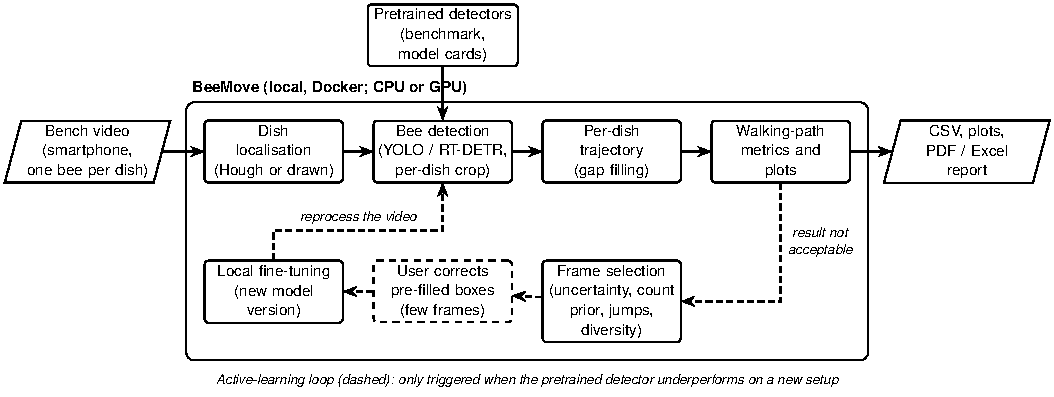
\includegraphics[width=\textwidth]{figures/Fig1.pdf}
\caption{Concept of \beemove. Solid arrows: analysis of a video with a pretrained detector. Dashed arrows: the active-learning loop, used only when the result on a new setup is not acceptable; the user corrects a few frames whose boxes come pre-filled by the current model}\label{fig:concept}
\end{figure}

\subsection{From video to trajectories}\label{sec:pipeline}

\paragraph{Frame sampling.} Videos are decoded in a background thread that feeds a bounded queue, so decoding and inference run concurrently; the user chooses a sampling step and, optionally, a time window. Frame indices always refer to the original video, so timestamps remain exact when frames are skipped.

\paragraph{Dish localisation.} Dishes are located automatically with the circular Hough transform on the first frame, or drawn by the user as circles or polygons; the user confirms them before processing. Dishes receive stable names (row by row, left to right), so the same arrangement yields the same labels across videos.

\paragraph{Detection.} \beemove{} accepts any detector trained with the Ultralytics framework, either a YOLO model or RT-DETR; the model class is chosen from the family declared in the model card, not from the file name. In \emph{zoom} mode the detector runs on a crop around each dish instead of the full frame, which enlarges the bee relative to the network input --- the median bee covers about 16 pixels at a 640-pixel input in our data. Because a crop includes a margin, a detection is accepted only if its centre lies inside that dish and outside all others.

\paragraph{Identity and gap filling.} The dish defines the identity of the trajectory: in each frame the most confident detection inside a dish is assigned to it and detections outside all dishes are discarded as false positives. Short gaps of a few sampled frames are filled by linear interpolation and flagged as such; longer gaps are left as missing data. Without dishes (open arenas), a greedy nearest-neighbour association links up to $N$ detections across frames.

\subsection{Walking-path metrics}\label{sec:metrics}

For a trajectory $\{(t_k, \mathbf{p}_k)\}_{k=1}^{K}$ of detection centres $\mathbf{p}_k$ at times $t_k$, \beemove{} reports the travelled distance $D=\sum_{k}\lVert\mathbf{p}_{k+1}-\mathbf{p}_k\rVert$, the net displacement $\lVert\mathbf{p}_K-\mathbf{p}_1\rVert$, the straightness index (net displacement over $D$), mean and maximum speed, and the time spent moving or stopped, where a step shorter than a threshold is counted as stopped to absorb detector jitter. Distances are in pixels by default and in millimetres when the user calibrates the scale on a frame (for example, along the known diameter of the dish). These descriptors follow standard trajectory analysis~\cite{benhamou2004how,mclean2018trajr}. Seven plots accompany the metrics: trajectory over time, heat map (masked to the region that holds 95\% of the occupancy mass, so the walked path remains visible when the bee rests in one spot), explored area, speed over time, cumulative distance, speed histogram and position over time. User-drawn zones add time in zone, number of visits and distance inside each zone, computed per trajectory.

\todo{Add one figure with real output of the tool (the seven plots for one dish of the example video) once the app runs on the new package; Fig5.}

\subsection{Architecture and deployment}\label{sec:architecture}

Figure~\ref{fig:architecture} shows the software architecture. A single Python package, \texttt{beemove}, contains the logic: detector loading, dish localisation, tracking, video reading, analytics, dataset building, fine-tuning, model cards and the active-learning strategies. Two programs import it. The \emph{research pipeline} builds the splits, trains and evaluates the detectors and runs the active-learning simulation on a laboratory GPU. The \emph{\beemove{} application}, written in Streamlit, provides accounts and analysis history, video upload, dish and zone definition, the annotation screen for suggested frames, background fine-tuning and reports.

\begin{figure}[t]
\centering
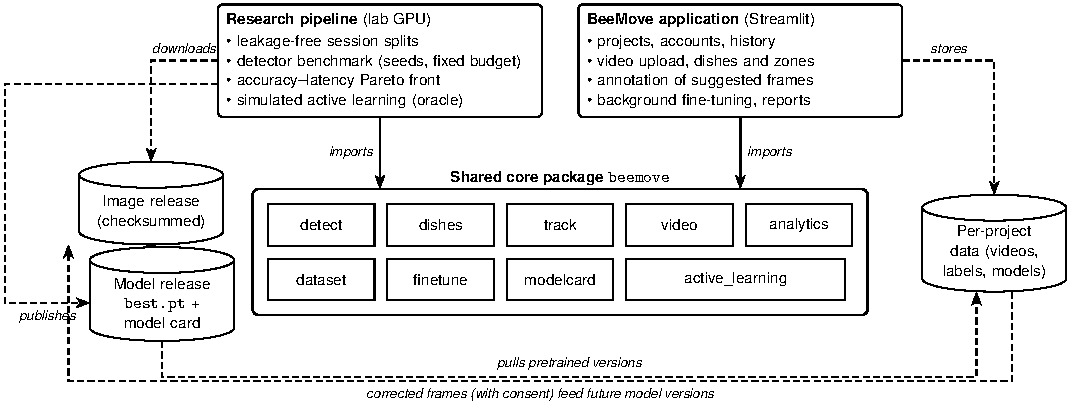
\includegraphics[width=\textwidth]{figures/Fig2.pdf}
\caption{Software architecture. The research pipeline and the application import the same package, so the experiments evaluate the code that users run. Models are distributed as a pair of weights and model card; corrected frames can, with consent, become training data for future model versions}\label{fig:architecture}
\end{figure}

Each distributed model is a pair formed by the weights and a \emph{model card}, a JSON file with the detector family and architecture, the training origin (protocol, fold, seed and a fingerprint of the training recipe), the framework version, the input size, the validation and test metrics, and the confidence threshold selected on validation. The application uses this threshold by default, so users start from the operating point reported in this paper. Pretrained models and the image set are published as checksummed releases and downloaded on first use.

\beemove{} runs entirely on the user's machine: videos never leave the laboratory. It is distributed as Docker images for CPU and GPU; on a CPU-only computer it analyses videos with the pretrained detectors, and fine-tuning uses the GPU when one is available. \todo{Report CPU fine-tuning time for a typical round, or state that fine-tuning requires a GPU.}

%% =====================================================================
\section{Active-learning loop}\label{sec:al}
%% =====================================================================

When the pretrained detector underperforms on a new setup, the user asks \beemove{} for frames to correct. The loop has four steps: (i) the current model scores a pool of frames sampled across the videos of the project; (ii) a strategy ranks them and proposes a batch of $b$ frames (by default, one crop per dish and frame); (iii) the user saves, adjusts or deletes the pre-filled boxes, or marks the dish as empty; (iv) the model is fine-tuned on all frames labelled so far, starting from the current weights, and the project videos are reprocessed. Each round produces a new model version with its own model card, so the user can compare versions and roll back.

\subsection{Selection strategies}\label{sec:strategies}

Because each dish holds exactly one bee, the setting offers cues that generic object detection lacks. \beemove{} implements the following strategies, all independent of the detector architecture:

\begin{itemize}
\item \textbf{Random} and \textbf{uniform in time}: baselines; the latter spreads the batch evenly over the video.
\item \textbf{Least confidence}: dishes whose best detection has the lowest score.
\item \textbf{Count prior}: dishes with zero or with two or more detections above a low threshold, which are certainly wrong for a single bee.
\item \textbf{Trajectory jumps}: frames where the detected position moves farther than a bee can walk between two sampled frames.
\item \textbf{Flip consistency}: disagreement between detections on the frame and on its mirrored copy.
\item \textbf{Committee disagreement}: disagreement among the pretrained detectors of different families.
\item \textbf{Diversity}: $k$-means over image embeddings of the detector backbone, choosing one frame per cluster, alone or combined with an uncertainty score (hybrid).
\end{itemize}

\todo{Keep only the strategies actually implemented and evaluated; define each score formally (equations) once beemove.active\_learning is written.}

\subsection{Fine-tuning recipe}\label{sec:finetune}

Fine-tuning reuses the training recipe of the benchmark with every hyper-parameter set explicitly, so that results do not depend on library defaults that change across versions. Labelled frames are split into training and validation by blocks of consecutive frames, never at random, because neighbouring frames are near duplicates. Frames marked as empty become negative examples. \todo{Number of epochs and early stopping for fine-tuning rounds, after the pilot runs.}

%% =====================================================================
\section{Data and evaluation protocol}\label{sec:protocol}
%% =====================================================================

\subsection{Dataset}\label{sec:dataset}

We reuse the 930 labelled images of our previous study~\cite{lima2025analyzing}: frames extracted from smartphone videos of bees walking in Petri dishes, at four resolutions ($1440^2$, $1080^2$, $1080\times1920$ and $1920\times1080$ pixels), with one bounding box per bee. Frames were sampled from 10-min videos of one bee per Petri dish filmed with smartphones about 30~cm above the dish, and annotated with bounding boxes~\cite{lima2025analyzing}. \todo{Species, compounds and doses; frame rate.} The original split kept each video in a single partition~\cite{lima2025analyzing}. Videos, however, were recorded in sessions in which the phone stays on the same support and only the dishes are exchanged, so videos of the same bench, background and lighting fell into different partitions; image matching also showed that the validation mosaics reuse footage of training videos. A detector evaluated this way is tested on scenes it has already seen. % NOTE (authors): evidence in bee-tracker docs/SESSOES_EVIDENCIAS.md; confirm wording before submission.

We therefore regrouped the 568 single-dish frames into nine \emph{recording sessions} (Table~\ref{tab:sessions}): frames from the same bench, camera position and background belong to the same session. Sessions were defined from the clip metadata and confirmed by image matching (SIFT keypoints with RANSAC) between clips, with three independent readings of the contact sheets. The sessions fall into two bench \emph{setups}: wooden blocks (W, five sessions, 328 frames) and plastic trays (P, four sessions, 240 frames). Synthetic mosaics present in the original release are excluded from the splits whenever their source frames span more than one session.

\begin{table}[t]
\caption{Recording sessions used to build leakage-free splits}\label{tab:sessions}
\begin{tabular*}{\textwidth}{@{\extracolsep\fill}lcccl}
\toprule
Session & Setup & Clips & Frames & Scene \\
\midrule
S01 & W & 3 & 90 & wooden blocks, $1440^2$ frames \\
S02 & W & 1 & 30 & wooden blocks, different arrangement \\
S03 & W & 3 & 88 & wooden blocks, landscape \\
S04 & W & 3 & 90 & wooden blocks, $1440^2$ frames \\
S05 & W & 1 & 30 & wooden blocks, portrait \\
S06 & P & 3 & 80 & plastic boxes, portrait \\
S07 & P & 3 & 70 & plastic trays, fixed camera \\
S08 & P & 2 & 60 & plastic tray \\
S09 & P & 1 & 30 & plastic tray, portrait \\
\midrule
Total & & 20 & 568 & \\
\botrule
\end{tabular*}
\end{table}

\subsection{Splits}\label{sec:splits}

Figure~\ref{fig:splits} shows the three protocols. \emph{5-fold by session} assigns whole sessions to test, validation and training in each fold. \emph{Leave one session out} (LOSO) holds out one session at a time and measures generalisation to an unseen recording. \emph{Cross setup} trains on one setup and tests on the other, which approximates a new laboratory. A script checks every split for image matches across partitions.

\begin{figure}[t]
\centering
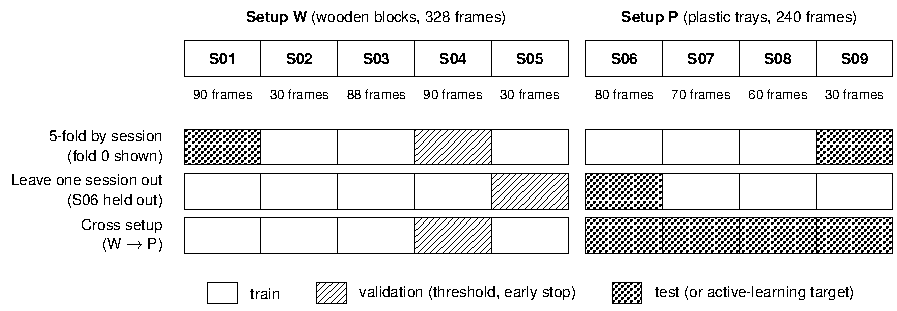
\includegraphics[width=\textwidth]{figures/Fig4.pdf}
\caption{Recording sessions and the three evaluation protocols. Patterns mark the role of each session in the example fold: plain for training, hatched for validation and dotted for test (or the target of the active-learning simulation)}\label{fig:splits}
\end{figure}

\subsection{Detector benchmark}\label{sec:benchmark}

We compare nine detectors available in the Ultralytics framework (version 8.4.69): the nano and small variants of YOLOv8~\cite{jocher2023ultralytics}, YOLO11~\cite{khanam2024yolov11}, YOLO12~\cite{tian2025yolov12} and YOLO26~\cite{jocher2026ultralytics}, and RT-DETR-L~\cite{zhao2024detrs}. All start from COCO weights and use the same explicit recipe: 150 epochs with early stopping on validation, input size 640, batch 8, AdamW with initial learning rate 0.002 and the warm-up and augmentation settings fixed in the configuration; RT-DETR uses a learning rate of $10^{-4}$ and batch 4, as recommended for transformer detectors. Each configuration is trained with three seeds per fold. Batch sizes reduced automatically by the framework when memory runs out are recorded and reported.

We report COCO-style AP at IoU 0.50:0.95, AP$_{50}$ and AP$_{75}$ on the test sessions, and precision, recall and F1 at the confidence threshold that maximises F1 on validation --- the operating point that the tool uses. Latency is measured end to end (image loading, pre-processing, inference and post-processing) on a fixed list of test images, on a CPU-only computer and on a modest GPU, as well as the network forward pass alone. Models on the Pareto front of accuracy versus CPU latency are released as the pretrained models of \beemove.

\subsection{Active-learning simulation}\label{sec:alsim}

Figure~\ref{fig:alsim} shows how the loop is evaluated without user effort: a ground-truth oracle plays the user and reveals the boxes of the frames each strategy selects. We consider three scenarios: \emph{new setup} (train on W, adapt to P, and vice versa), \emph{new session} (LOSO) and \emph{no prior model} (start from COCO weights). In each round the strategy selects $b$ frames from the unlabelled pool of the target, the model is fine-tuned on all frames labelled so far and evaluated on held-out target sessions that are never queried. We plot AP and the error on walking-path metrics against the number of labelled frames, with \todo{5} seeds per strategy, and compare every strategy with random selection, which is a strong baseline in realistic active-learning evaluations~\cite{munjal2022towards,luth2023navigating}. \todo{Initial budget, batch size $b$ and maximum budget after the pilot (plan: start with 10--20 frames, 5--10 per round, up to about 150).}

\begin{figure}[t]
\centering
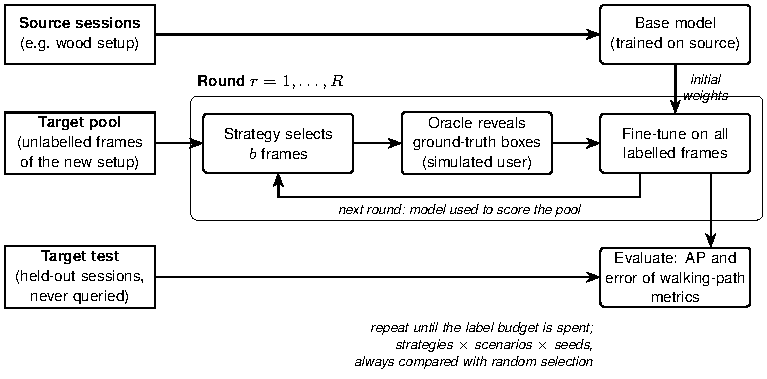
\includegraphics[width=0.85\textwidth]{figures/Fig3.pdf}
\caption{Simulated active-learning protocol. A ground-truth oracle stands in for the user; target test sessions are never queried. The loop is repeated until the label budget is spent, for each strategy, scenario and seed}\label{fig:alsim}
\end{figure}

\subsection{Effect on walking-path metrics}\label{sec:metricerror}

Detection accuracy matters to users only through the metrics they read. We therefore annotate the centre of the bee in continuous stretches of \todo{N} videos, without looking at the model output, and measure the error of distance, mean speed and time stopped computed from \beemove{} trajectories with respect to these references, before and after each active-learning round. Agreement is reported with Bland--Altman limits of agreement~\cite{bland1986statistical} rather than correlation, because the question is whether the tool can replace the reference measurement. \todo{Confirm availability of continuous videos (at least one is available) and of new setups from other laboratories.}

\subsection{Research questions}\label{sec:rq}

\begin{description}
\item[RQ1] Which detectors offer the best trade-off between accuracy and CPU latency for this task when evaluated without leakage?
\item[RQ2] How much does accuracy drop on an unseen session or bench setup?
\item[RQ3] How many corrected frames does the loop need to recover that drop, and do the arena-specific strategies beat random selection?
\item[RQ4] How do detection errors translate into errors of walking-path metrics?
\end{description}

%% =====================================================================
\section{Results}\label{sec:results}
%% =====================================================================

\subsection{Detector benchmark (RQ1)}

\result{Table: AP, AP$_{50}$, F1 at the validation threshold, end-to-end CPU and GPU latency, parameters and GFLOPs, mean $\pm$ standard deviation over folds and seeds (source: results/session\_v1/kfold5/REPORT.md). Figure: Pareto front of AP versus CPU latency.}

\subsection{Generalisation to new sessions and setups (RQ2)}

\result{LOSO and cross-setup AP compared with the 5-fold results; per-session breakdown.}

\subsection{Active learning (RQ3)}

\result{Learning curves (AP versus labelled frames) per scenario and strategy, with confidence bands over seeds; frames needed to reach 95\% of the in-domain AP; area under the curve compared with random selection.}

\subsection{Walking-path metrics (RQ4)}

\result{Error of distance, speed and time stopped versus reference trajectories, before and after adaptation.}

%% =====================================================================
\section{Discussion}\label{sec:discussion}
%% =====================================================================

\todo{Interpretation of RQ1--RQ4; practical guidance (which model on a CPU, how many frames to correct).}

\paragraph{Threats to validity.} The dataset comes from one research group and two bench setups, and frames, not continuous videos, carry the box annotations; the simulation assumes a perfect oracle, whereas users make mistakes and take time; the number of sessions limits the statistical power of between-model comparisons, so we report dispersion over folds and seeds and avoid claims that it does not support. \todo{Usability study with researchers from other laboratories, if carried out.}

%% =====================================================================
\section{Conclusion}\label{sec:conclusion}
%% =====================================================================

\todo{Summary of the tool and of the findings; future work: multi-animal arenas, identity across dishes, other insects, a hosted version.}

%% =====================================================================
\backmatter

\bmhead{Acknowledgements}
\todo{People and institutions; funding agencies in full.}

\section*{Statements and Declarations}

\bmhead{Funding}
\todo{Funding statement with agency names in full and grant numbers, or ``No funding was received for conducting this study.''}

\bmhead{Competing interests}
The authors have no competing interests to declare that are relevant to the content of this article. \todo{confirm}

\bmhead{Ethics approval}
\todo{Bees are invertebrates; state whether an ethics committee approval was required. If the species is native to Brazil, add the SISBIO/SisGen registration if applicable. If a usability study with researchers is run, add the human-participants statement and informed consent.}

\bmhead{Data availability}
The images, annotations, session manifest and splits are available at \todo{Zenodo DOI}. The images are those of a previous study~\cite{lima2025analyzing}.

\bmhead{Code availability}
The \beemove{} source code, the research pipeline and the pretrained models with their model cards are available at \todo{repository URL and Zenodo DOI} under the \todo{licence; the package is declared AGPL-3.0 because it depends on Ultralytics}.

\bmhead{Use of generative AI}
\todo{MTAP requires documenting the use of large language models beyond copy editing in the Methods section. Parts of the software and of this draft were produced with the assistance of an AI coding assistant; describe what it was used for and confirm human accountability, or remove if not applicable.}

\bmhead{Author contributions}
\todo{CRediT statement.}

%% =====================================================================
\bibliography{references}

\end{document}
